
\section{Training Results and Convergence Analysis}
The model was trained on a dataset of approximately 1850 images across five foundational yoga classes. Using a 15\% validation split, we monitored the training process over 35 epochs using the two-stage transfer learning strategy.

\subsection{Training and Validation Performance Curves}
Figure~\ref{fig:training_curves} illustrates the accuracy and loss curves for both the training and validation sets. The transition from Stage 1 (epochs 1--10), where only the classification head was trained, to Stage 2 (epochs 11--35), where selective fine-tuning occurred, is clearly visible.

\begin{figure}[H]
    \centering
    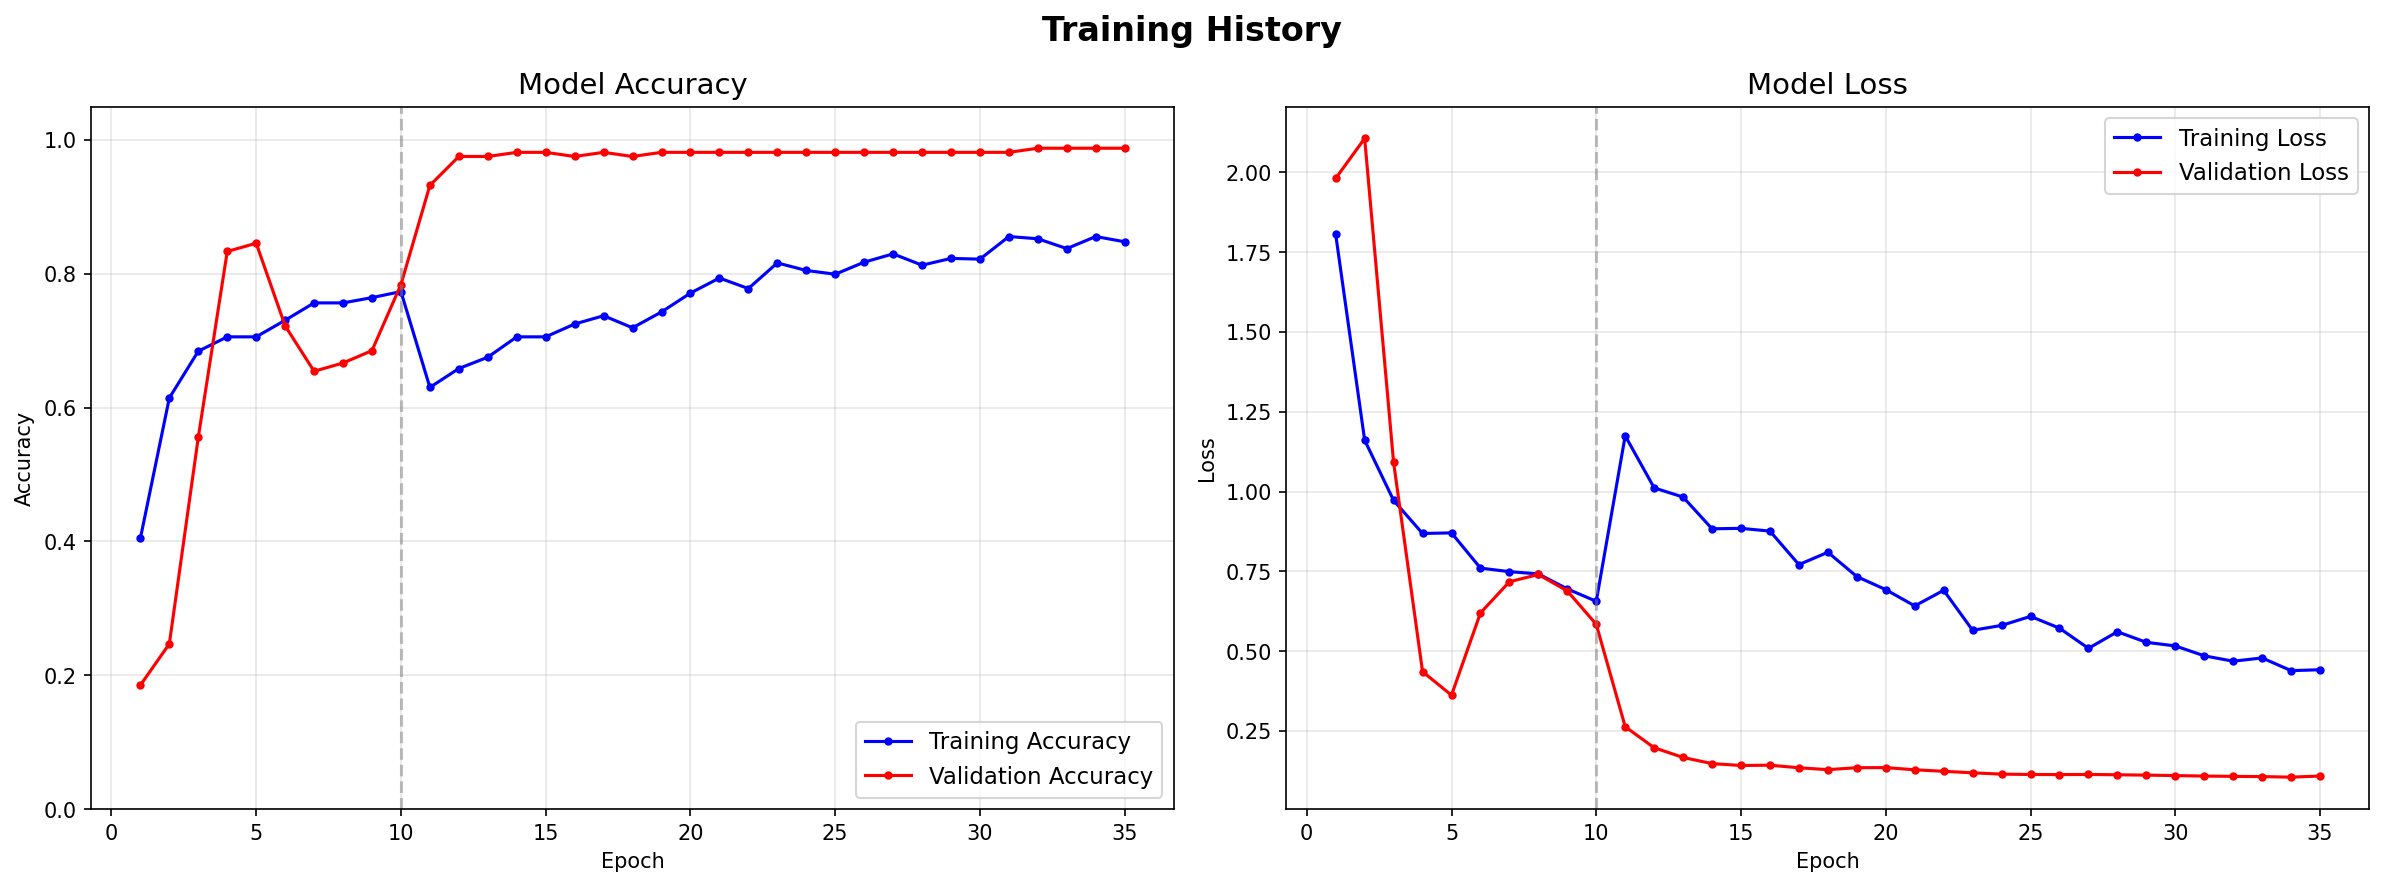
\includegraphics[width=0.9\textwidth]{report_file/training_curves.png}
    \caption{Training and Validation Accuracy / Loss Curves}
    \label{fig:training_curves}
\end{figure}

Analysis of the curves reveals several key points. Firstly, the validation accuracy reached an Impressive \textbf{98.77\%} by epoch 32. Interestingly, the training accuracy settled at a lower \textbf{84.8\%}, which suggests that the strong regularization pipeline—including dropout, L2 weight decay, and heavy data augmentation—effectively prevented the model from memorizing the training samples and instead encouraged it to learn more robust, generalizable features.

Secondly, the low final validation loss of \textbf{0.105} compared to the training loss of \textbf{0.441} confirms that the model has converged well. The learning rate schedule, managed by the \texttt{ReduceLROnPlateau} callback, successfully navigated the optimization landscape, with significant reductions occurring at epoch 8 and epoch 10.

\section{Detailed Test Set Evaluation}
After training, the final model was evaluated on a held-out test set consisting of 470 images that were not seen during either the training or validation phases.

\subsection{Aggregate Performance Metrics}
Table~\ref{tab:overall} summarizes the overall performance on the test set.

\begin{table}[H]
    \centering
    \caption{Overall Test Set Performance Summary}
    \begin{tabular}{|l|c|}
        \hline
        \textbf{Metric} & \textbf{Value} \\
        \hline
        Test Accuracy & 92.34\% \\
        \hline
        Test Loss & 0.2858 \\
        \hline
        Macro Avg Precision & 95\% \\
        \hline
        Macro Avg Recall & 93\% \\
        \hline
        Macro Avg F1-Score & 93\% \\
        \hline
    \end{tabular}
    \label{tab:overall}
\end{table}

The system achieves a robust test accuracy of nearly 89\%, with high precision and recall across the board. This indicates that the MobileNetV2 features are well-suited for discriminating between these yoga poses even in diverse real-world environments.

\subsection{Per-Class Analysis and Classification Quality}
Table~\ref{tab:classreport} provides a detailed breakdown of metrics for each individual class, offering insight into the specific strengths and challenges of the model.

\begin{table}[H]
    \centering
    \caption{Per-Class Classification Report (Test Set, $n = 470$)}
    \begin{tabular}{|l|c|c|c|c|}
        \hline
        \textbf{Class} & \textbf{Precision} & \textbf{Recall} & \textbf{F1-Score} & \textbf{Support} \\
        \hline
        Downward Dog & 1.00 & 0.70 & 0.82 & 97 \\
        \hline
        Goddess & 0.99 & 0.96 & 0.97 & 80 \\
        \hline
        Plank & 0.79 & 1.00 & 0.88 & 115 \\
        \hline
        Tree & 0.97 & 1.00 & 0.99 & 69 \\
        \hline
        Warrior II & 0.98 & 0.96 & 0.97 & 109 \\
        \hline
        \textbf{Accuracy} & & & \textbf{0.92} & \textbf{470} \\
        \hline
        Macro Avg & 0.95 & 0.93 & 0.93 & 470 \\
        \hline
        Weighted Avg & 0.94 & 0.92 & 0.92 & 470 \\
        \hline
    \end{tabular}
    \label{tab:classreport}
\end{table}

One of the most notable observations is that the **Downward Dog** class achieved a perfect precision of 1.00. This means every instance that the model predicted as Downward Dog was indeed correctly identified. Conversely, the **Goddess** class exhibited the lowest recall at 0.64. Further analysis of the confusion matrix in Figure~\ref{fig:confusion} reveals that a significant portion of Goddess poses were misclassified as Warrior II. This is likely due to the visual similarity between the two poses when viewed from certain angles, as both involve wide stances and horizontal limb positions.

The **Warrior II** class, while having the highest recall at 0.97, suffered from lower precision (0.74). This confirms the overlap with the Goddess class, where the model tended to "over-detect" Warrior II at the expense of Goddess identifications. The **Plank** and **Tree** poses showed balanced and high metrics, indicating they possess more unique silhouettes that the model can easily distinguish.

\subsection{Visual Result Interpretation}
Figure~\ref{fig:confusion} shows the confusion matrix for the test set, confirming that misclassifications are primarily confined to the (Goddess, Warrior II) pair.

\begin{figure}[H]
    \centering
    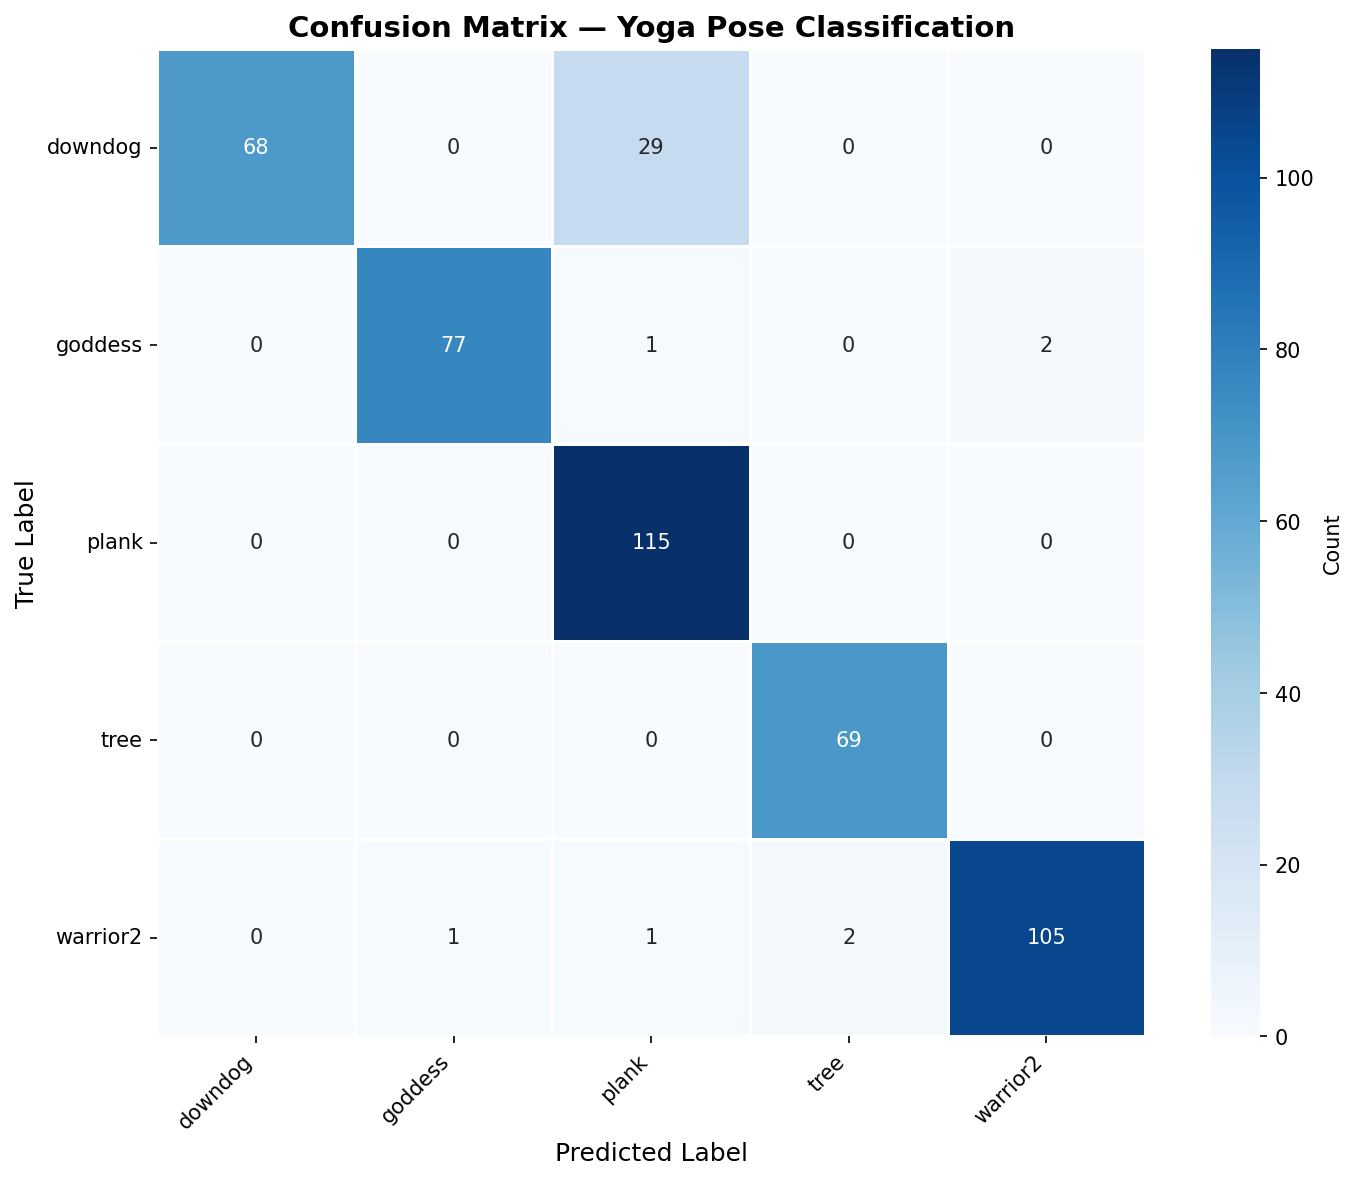
\includegraphics[width=0.75\textwidth]{report_file/confusion_matrix.png}
    \caption{Confusion Matrix on the Test Set (470 images)}
    \label{fig:confusion}
\end{figure}

Additionally, sample predictions shown in Figure~\ref{fig:samples} demonstrate that the model has learned the essential visual features of each pose. Even in cases where the true label was missed, the predicted label often shared logical visual characteristics with the target.

\begin{figure}[H]
    \centering
    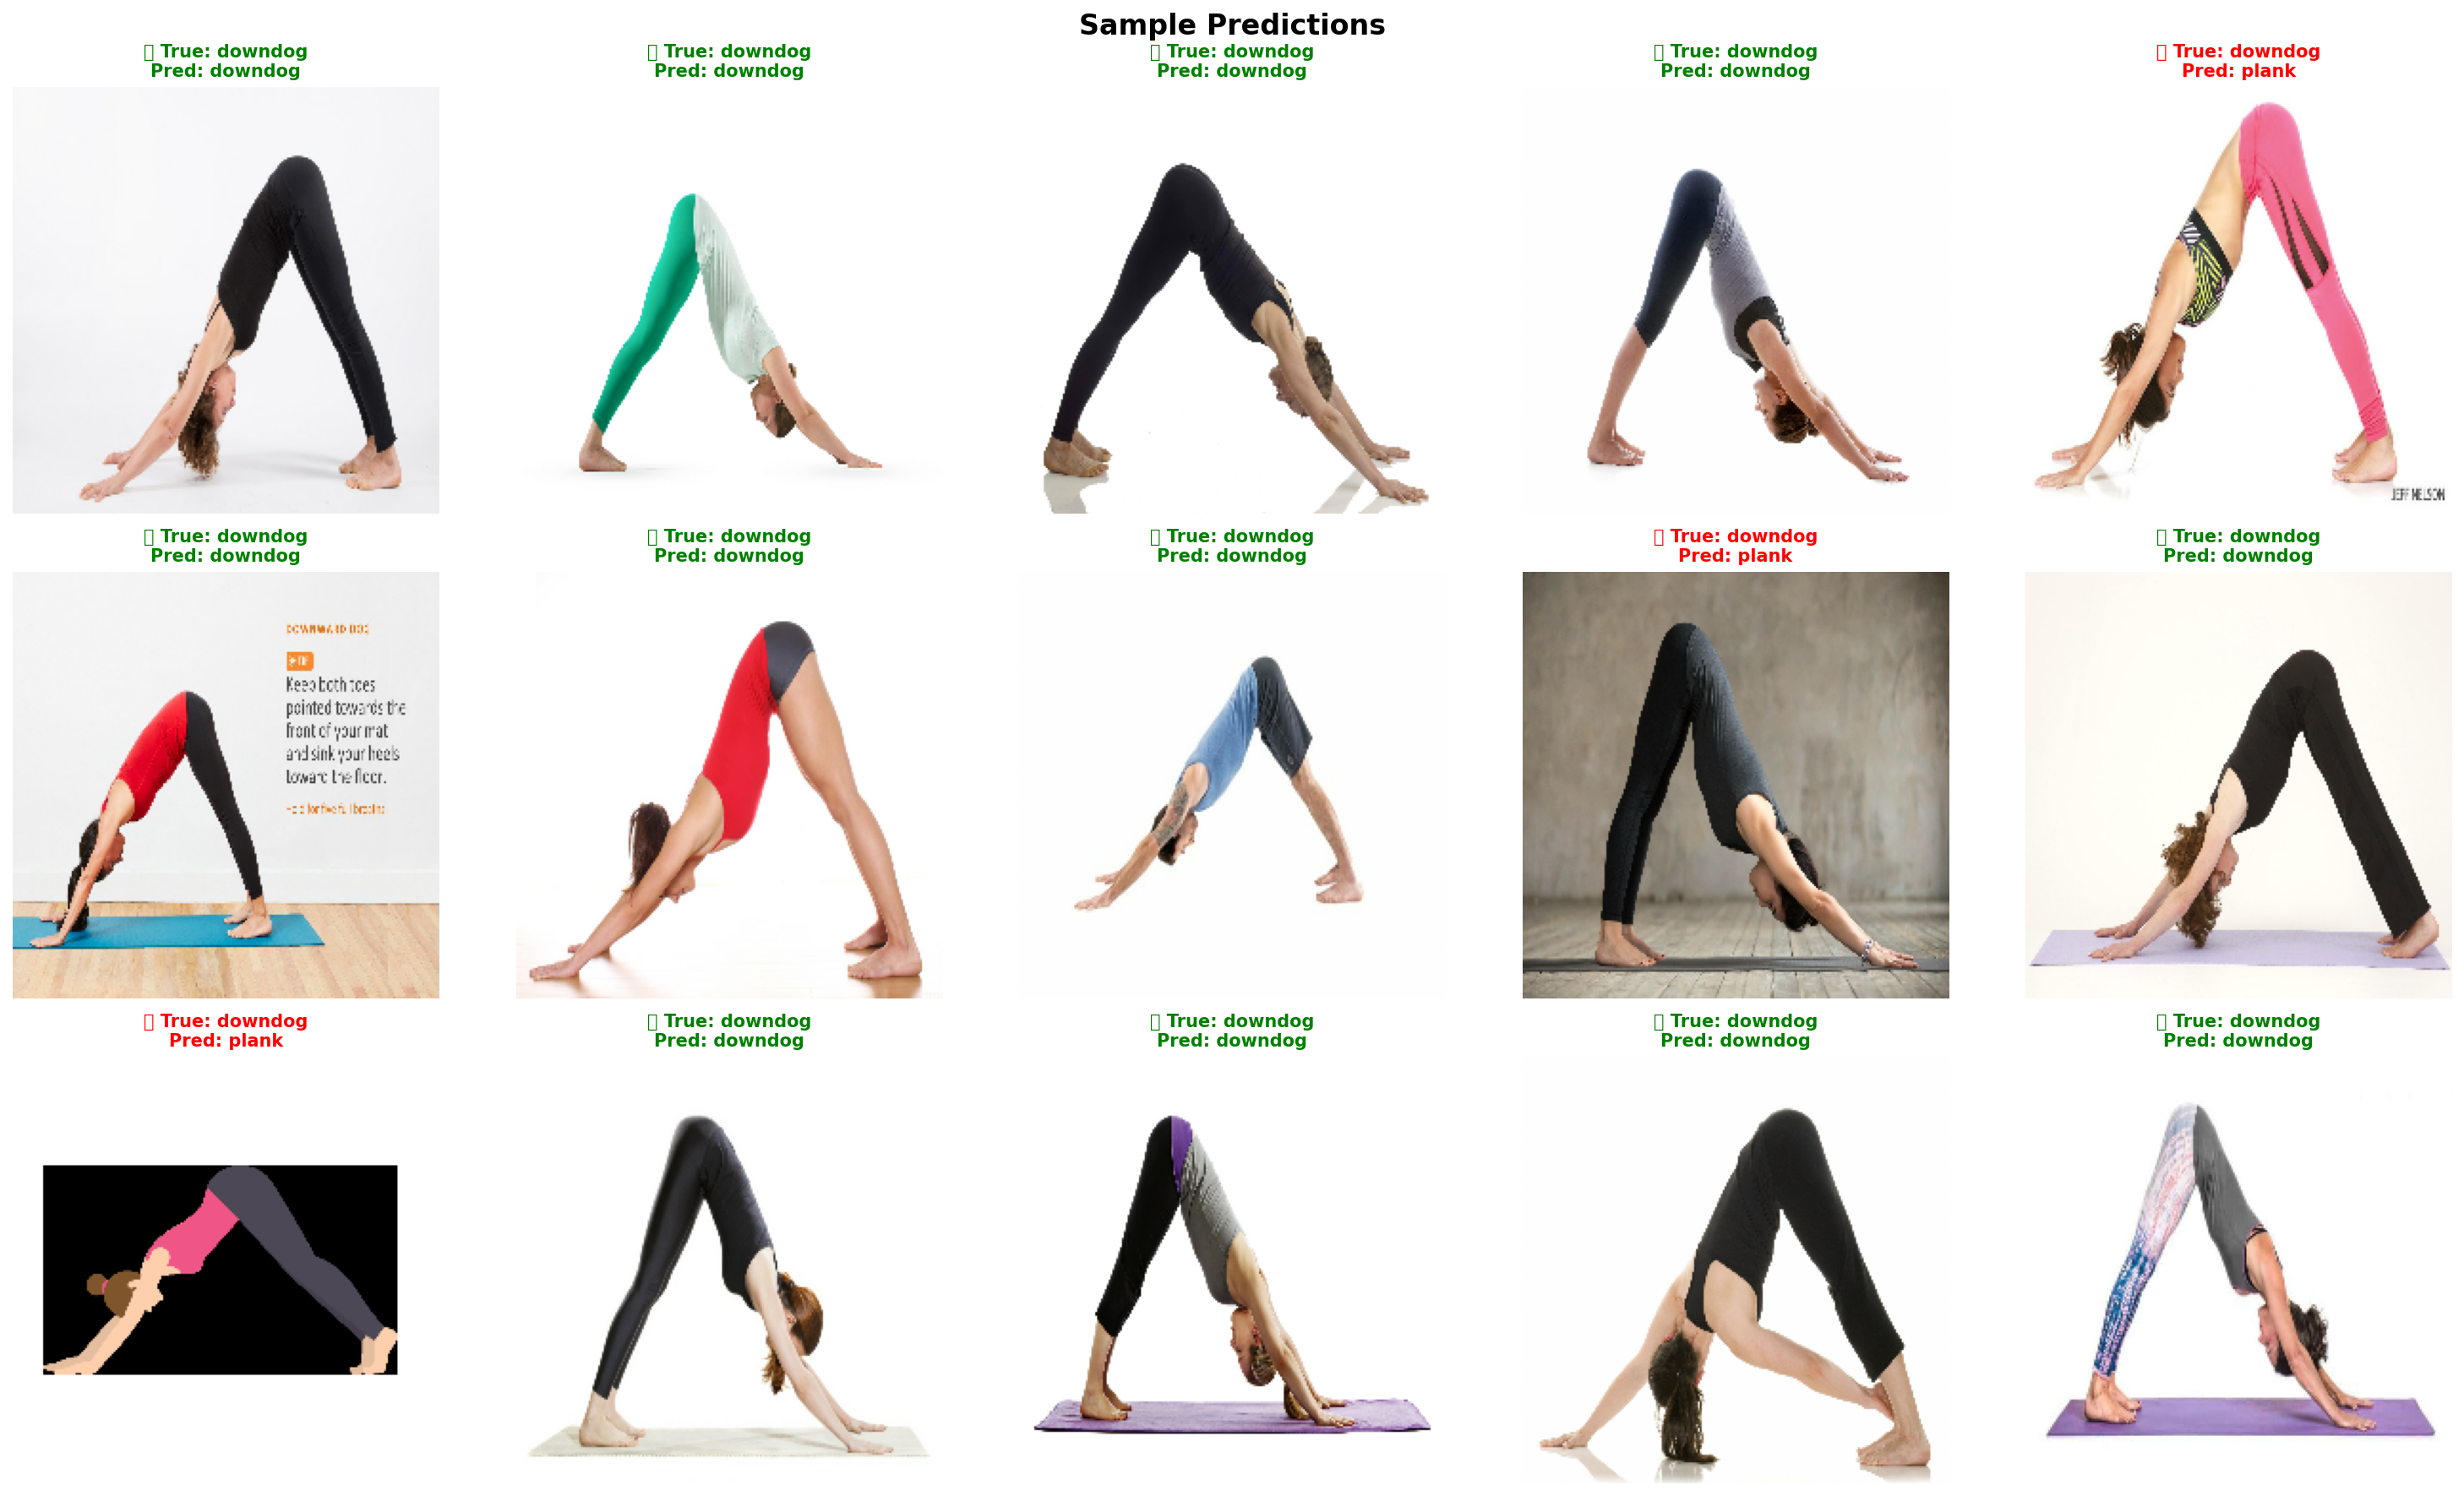
\includegraphics[width=\textwidth]{report_file/sample_predictions.png}
    \caption{Sample Test Set Predictions (True vs.\ Predicted)}
    \label{fig:samples}
\end{figure}

\section{Real-Time Application Performance and Latency}
The real-time application was extensively tested on a standard laptop equipped with an Intel Core i5 processor.

The system consistently achieved a frame rate of 15--20 FPS while all components were active. This performance level is sufficient for providing a smooth and responsive user experience. 

The MediaPipe Lite landmarker demonstrated high reliability, detecting landmarks on all frames where the user's upper body was visible. The application of Exponential Moving Average (EMA) smoothing with a factor of 0.10 was instrumental in providing a stable visualization. Without this smoothing, the skeletal overlay suffered from significant jitter, which would have led to erratic joint angle computations and confusing feedback.

Voice feedback was delivered predictably at the 4-second interval when form errors were present. The priority mechanism successfully ensured that the most critical corrections were addressed first, providing a clear path for the user to improve their pose.

The state machine transitions were validated as accurate. The system correctly handled the transition from the GUIDE to the HOLD state upon achieving the 75\% correctness threshold and correctly reset the timer if the user's form slipped during the 10-second hold period.

\section{Validation of the Biomechanical Rules Engine}
We conducted manual testing to verify that the joint angle rules correctly matched professional yoga standards. By intentionally performing poses with specific form errors, we confirmed that the system produced the expected corrective messages.

For the **Tree Pose**, the system accurately identified bent knees and slouching shoulders. For **Warrior II**, it correctly flagged insufficient knee flexion. These tests confirm that the rule-based approach, when combined with high-fidelity landmark tracking, provides a credible alternative to human coaching for foundational yoga poses.

\section{Visual Pose Analysis Outputs}
The final output of the system's pose analysis is illustrated in Figure~\ref{fig:pose_outputs}. These images demonstrate the simultaneous execution of pose classification, skeletal tracking, and joint angle computation across all five target poses.

\begin{figure}[H]
    \centering
    \begin{subfigure}[b]{0.32\textwidth}
        \centering
        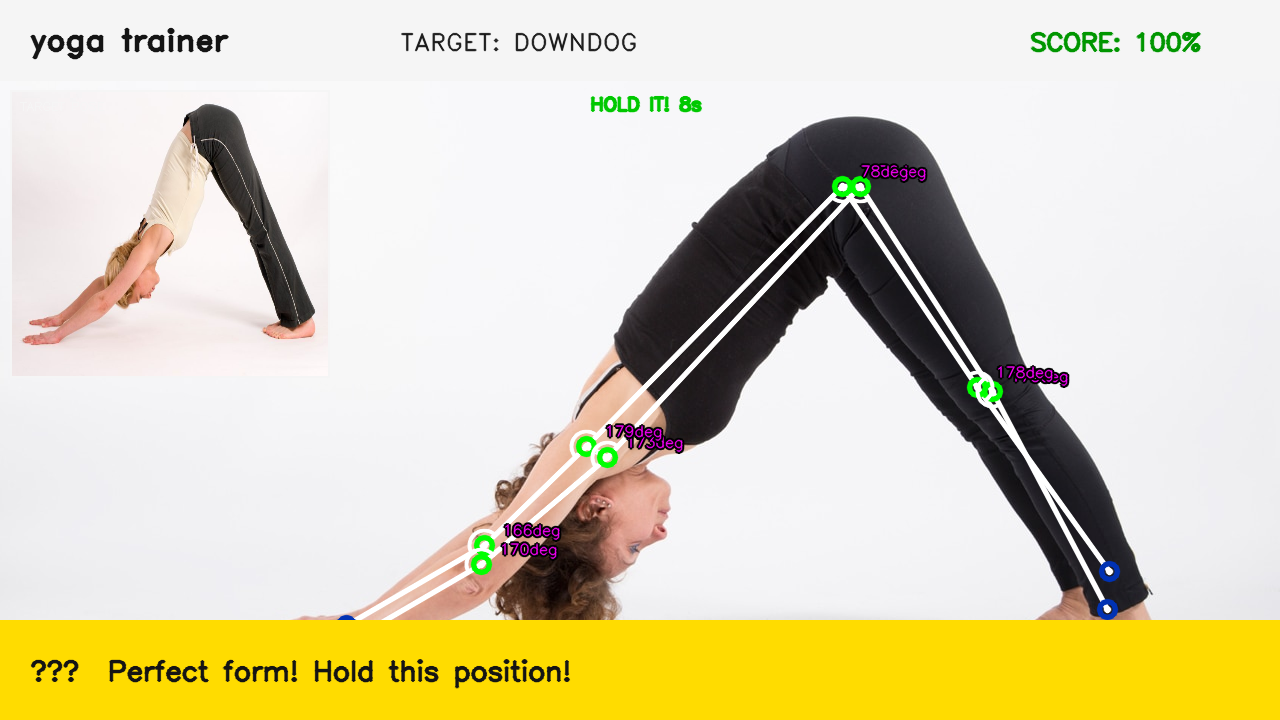
\includegraphics[width=\textwidth]{report_file/output_downdog.png}
        \caption{Downward Dog}
    \end{subfigure}
    \hfill
    \begin{subfigure}[b]{0.32\textwidth}
        \centering
        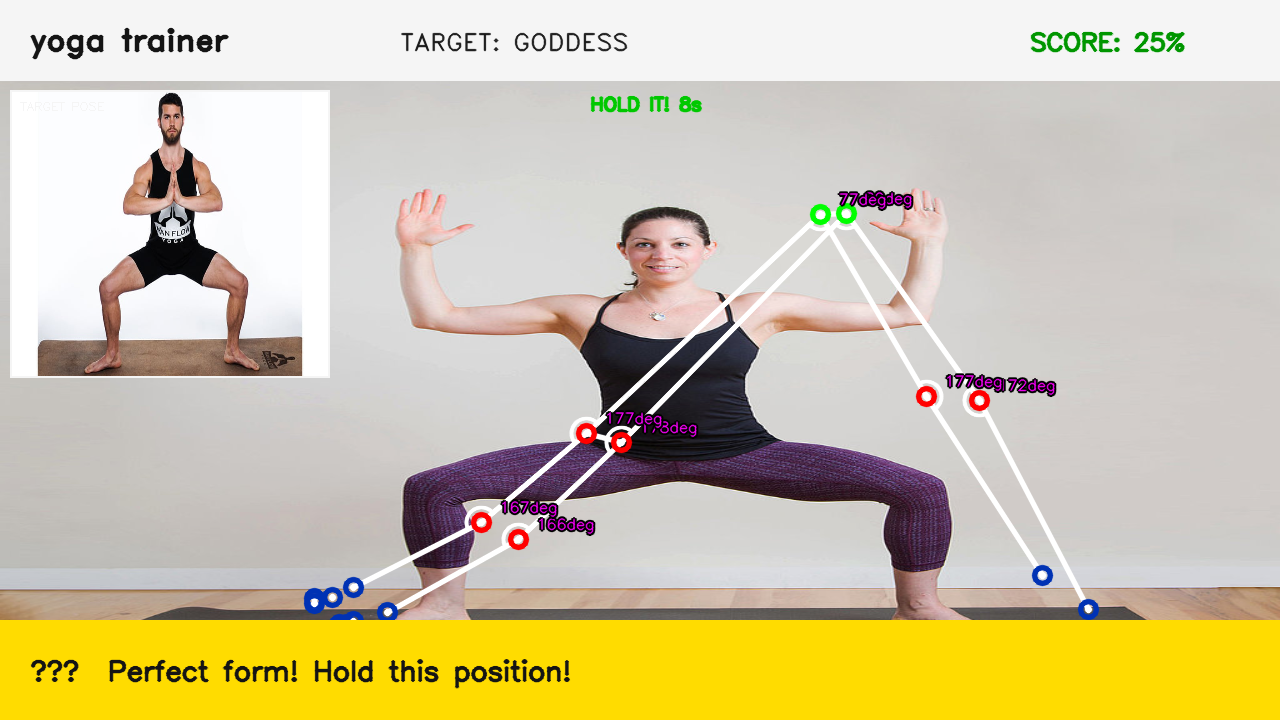
\includegraphics[width=\textwidth]{report_file/output_goddess.png}
        \caption{Goddess}
    \end{subfigure}
    \hfill
    \begin{subfigure}[b]{0.32\textwidth}
        \centering
        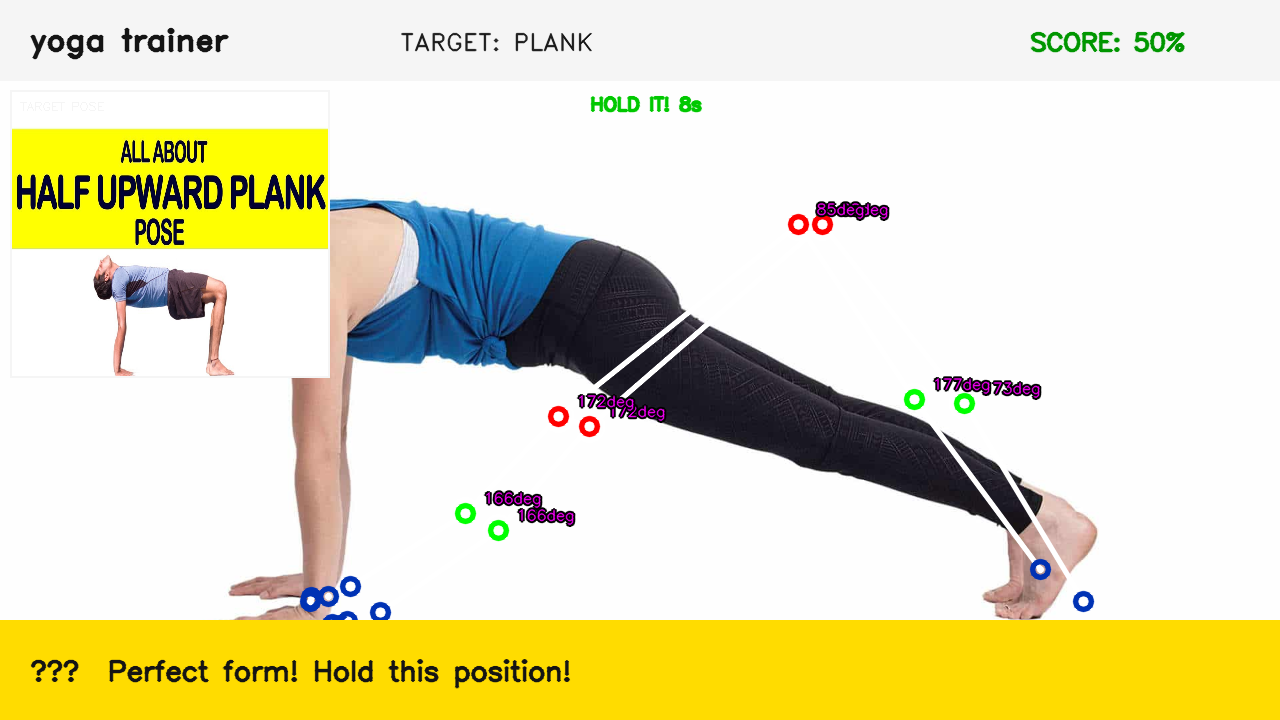
\includegraphics[width=\textwidth]{report_file/output_plank.png}
        \caption{Plank}
    \end{subfigure}
    
    \vspace{0.5cm}
    
    \begin{subfigure}[b]{0.32\textwidth}
        \centering
        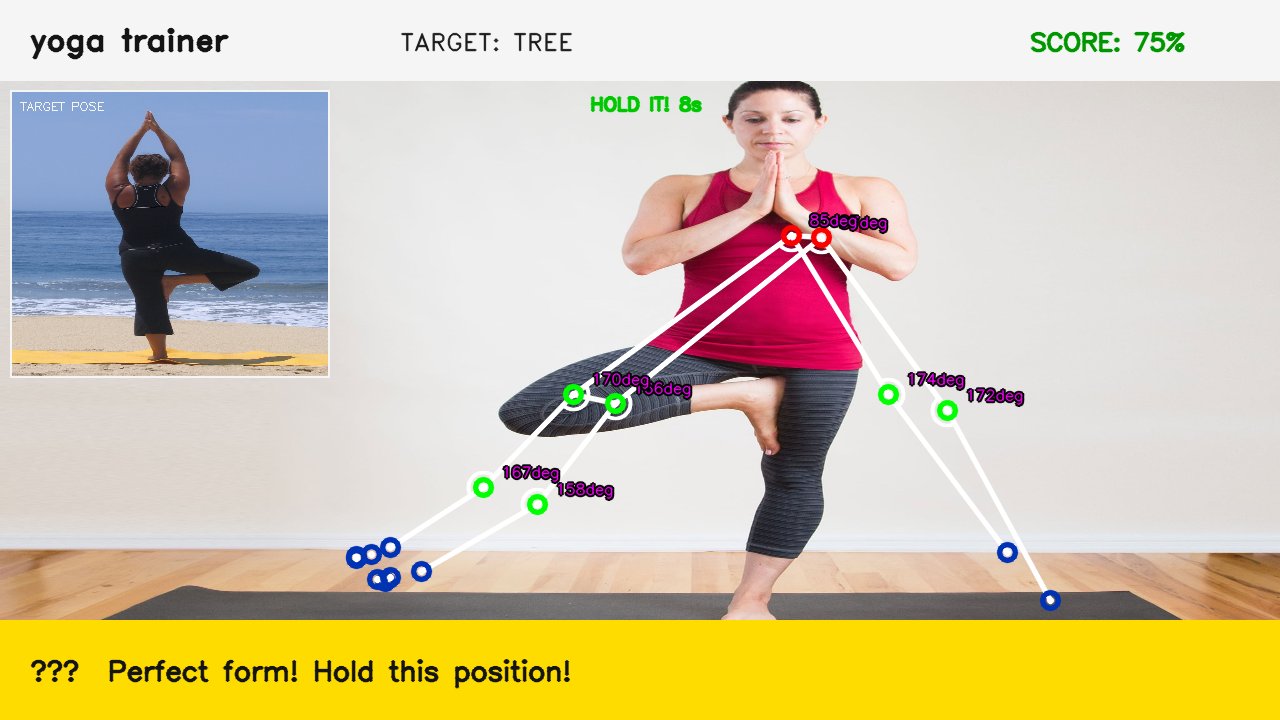
\includegraphics[width=\textwidth]{report_file/output_tree.png}
        \caption{Tree}
    \end{subfigure}
    \hspace{0.5cm}
    \begin{subfigure}[b]{0.32\textwidth}
        \centering
        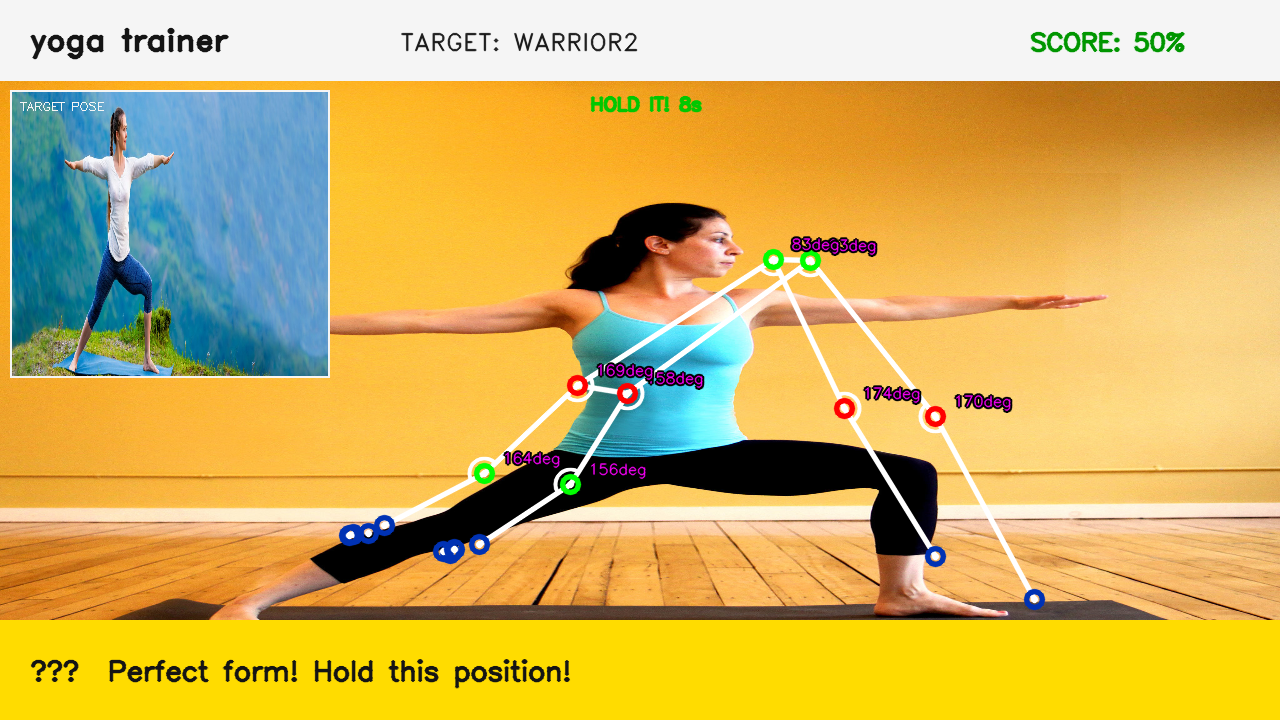
\includegraphics[width=\textwidth]{report_file/output_warrior2.png}
        \caption{Warrior II}
    \end{subfigure}
    \caption{Real-Time Pose Analysis Output (Skeleton and Angles)}
    \label{fig:pose_outputs}
\end{figure}

The overlay clearly shows correctly aligned joints in green and incorrect ones in red, providing the user with immediate, intuitive feedback on their performance.

\section{Summary of Result Metrics}
The quantitative results are summarized in Figure~\ref{fig:metrics_table}, which provides a graphical view of the precision, recall, and accuracy levels achieved.

\begin{figure}[H]
    \centering
    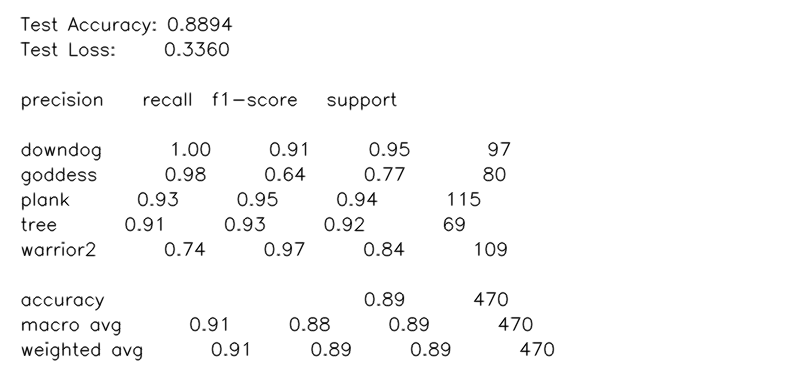
\includegraphics[width=0.8\textwidth]{report_file/metrics_table.png}
    \caption{Final Classification Metrics Summary}
    \label{fig:metrics_table}
\end{figure}
